\section{Selected Results on Alignment of the Tracking System with~2015 Data}
\label{sec:alignmentResults}

Different data-taking periods in 2015 include periods of cosmic ray data-taking with the magnetic field $B=0$T and $B=3.8$T, and periods of collision data-taking at $\sqrt{s}=13$~TeV center-of-mass energy with $B=0$T and $B=3.8$T. Different data-taking periods correspond to different detector geometries particularly due to changes of the magnetic field. 

Alignment constants have been derived for each data-taking period using the data collected during that period. Alignments under study are the result of a combination of a global (Millepede-II) and local (HIP) fit approach. The results are obtained by different approaches of running the two algorithms in sequence. In each data-taking period, the starting point for the alignment fit is the alignment obtained in the previous data-taking period. In addition, the two algorithms run independently confirm each other. 

The first alignment of the tracker, using~$B=0$T and~$B=3.8$T cosmic ray data, corrected for the shifts that took place since the end of Run~I of the LHC. The pixel modules in particular were repaired during the shutdown, and the pixel subdetectors were also recentered within the tracker. The tracker geometry changed between the~$B=3.8$T cosmic ray data and the first collisions, recorded with the magnetic field off, primarily because the changing magnetic field causes movements in the tracker. These effects are apparent mostly in the pixel detector, and the alignment performed using~$B=0$T collisions and cosmic rays (taken in between collision-data runs) recovers the tracker performance in the reconstruction of charged particle kinematic parameters. The tracker geometry changed again when the magnetic field was turned back on. New alignment constants are fitted for larger substructures of the pixel detector (BPIX half-barrels and FPIX half-cylinders) only. The changes, again produced by the changing magnetic field, are recovered by this alignment.

Validation of tracking system alignment tools include geometry comparison tool (Ch.~\ref{sec:AlRes_GCP}), validation using distribution of median residuals (Ch.~\ref{sec:AlRes_DMRs}), cosmic track splitting validation (Ch.~\ref{sec:AlRes_trackSplit}), and primary vertex validation (Ch.~\ref{sec:AlRes_PVvalid}). Full results of the first alignment with Run~II data are available at~\cite{ref_AlApproved_twiki}.

\subsection{Geometry Comparison}
\label{sec:AlRes_GCP}

Geometry Comparison is a visualization of the module-position differences of two different tracker geometries. Comparison of Run II and Run I positions of the modules in the forward-pixel (FPIX) detector of the tracker is shown in Fig.~\ref{fig:GCP_FPIX}. Each dot in Fig.~\ref{fig:GCP_FPIX} correspond to one module. The positions are determined with the Millepede-II and HIP algorithms using cosmic ray data collected with $B=0$T and $B=3.8$T magnetic field in the solenoid. The difference $\Delta z$ (Run~II~-~Run~I) as a functions of $z$ (left) and $\phi$ (right) in global coordinates. Four half-disks at the $-z$ side (four clusters of red dots at the left plot) are displaced by~-4.5~mm and~-5.5~mm. Much smaller relative movements of up to~200~$\mu$m are observed for the modules in the half-disks on the $+z$ side (two clusters of black dots). Shifted half-disks are shown as four clusters of red dots at the left plot and as shifted parts at ($\phi<-\pi/2$, $\phi>\pi/2$) and ($-\pi/2<\phi<\pi/2$) at the right plot. In addition to two-dimensional geometry comparison plots, three-dimentional plot of the pixel detector is also produced for better visuzlization (Fig.~\ref{fig:GCP_3D}).

\begin{figure}[htb]
    \begin{center}
        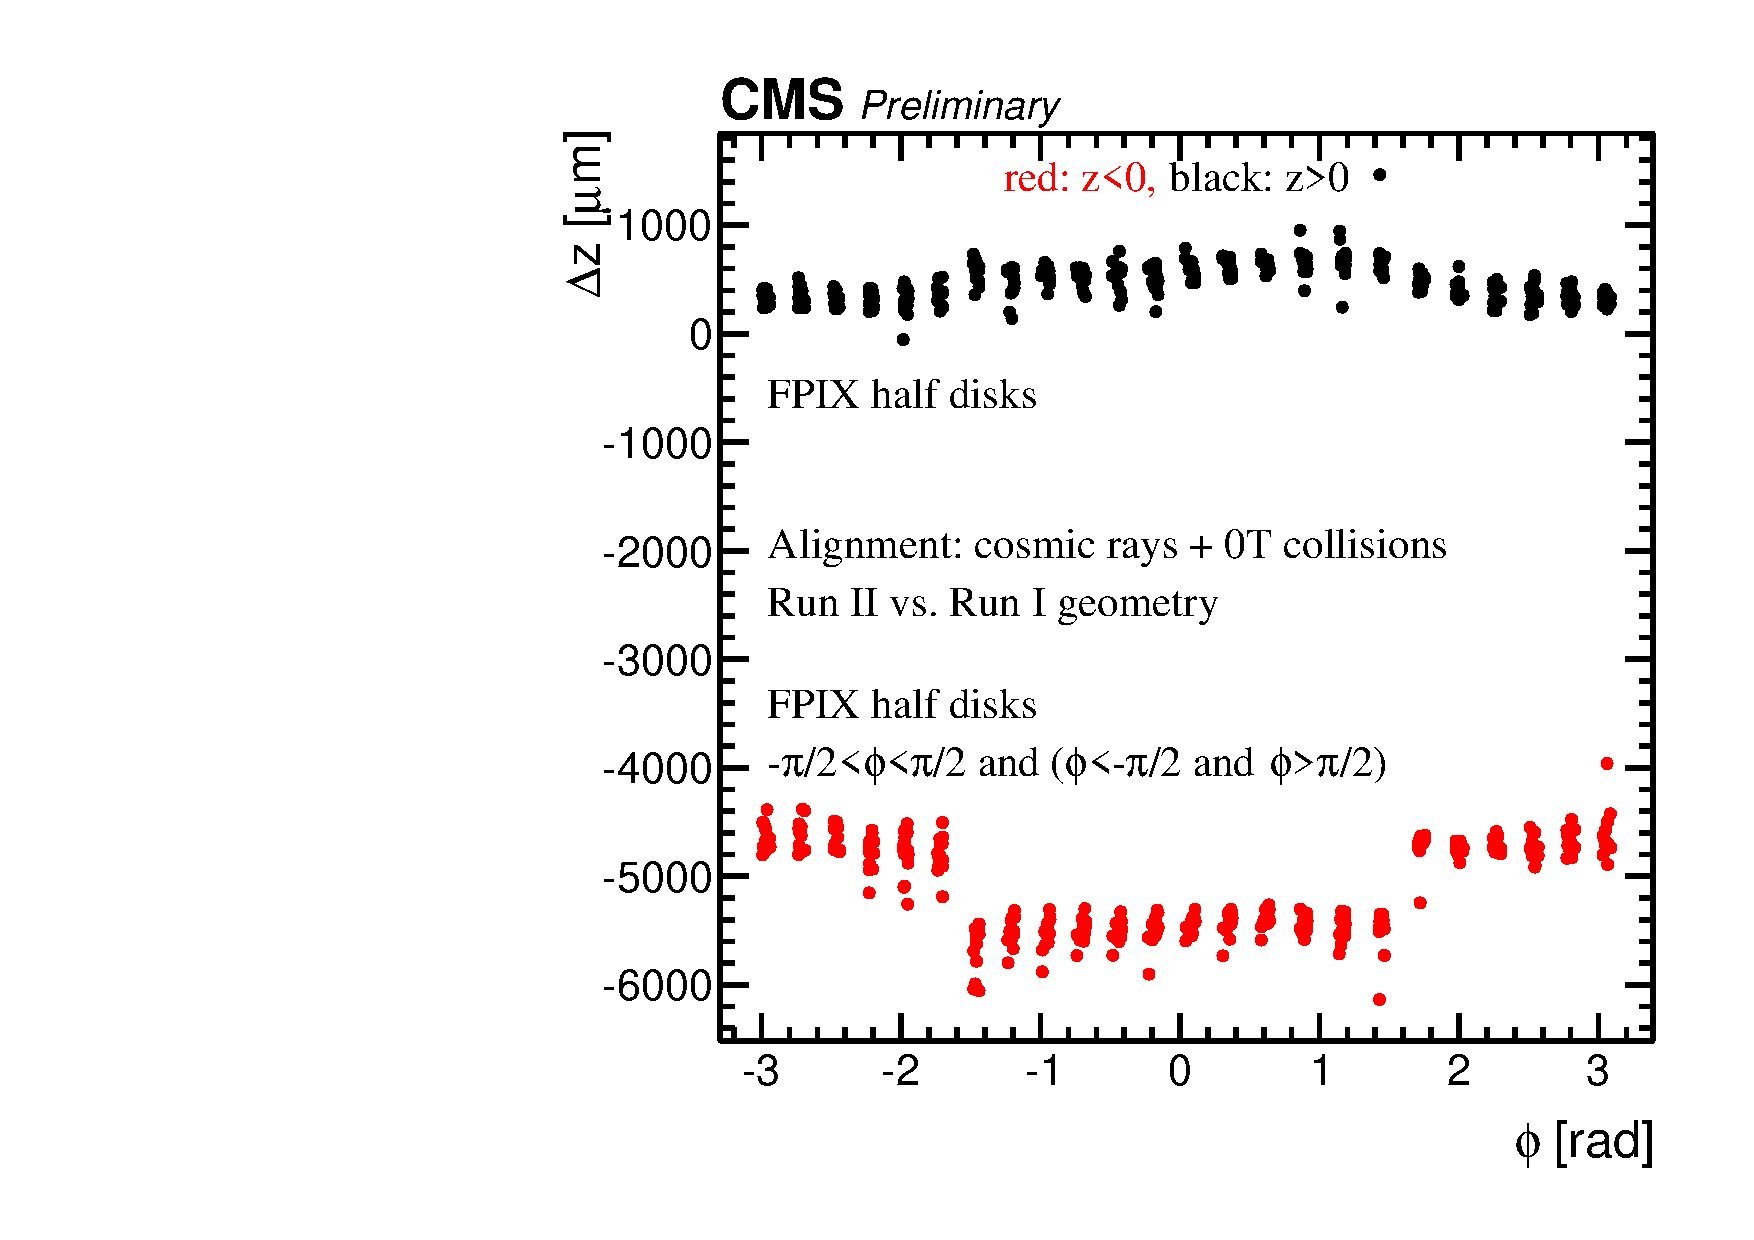
\includegraphics[width=0.45\textwidth]{../figs/Alignment/AlRes_phi_vs_dz_PXF_1.pdf}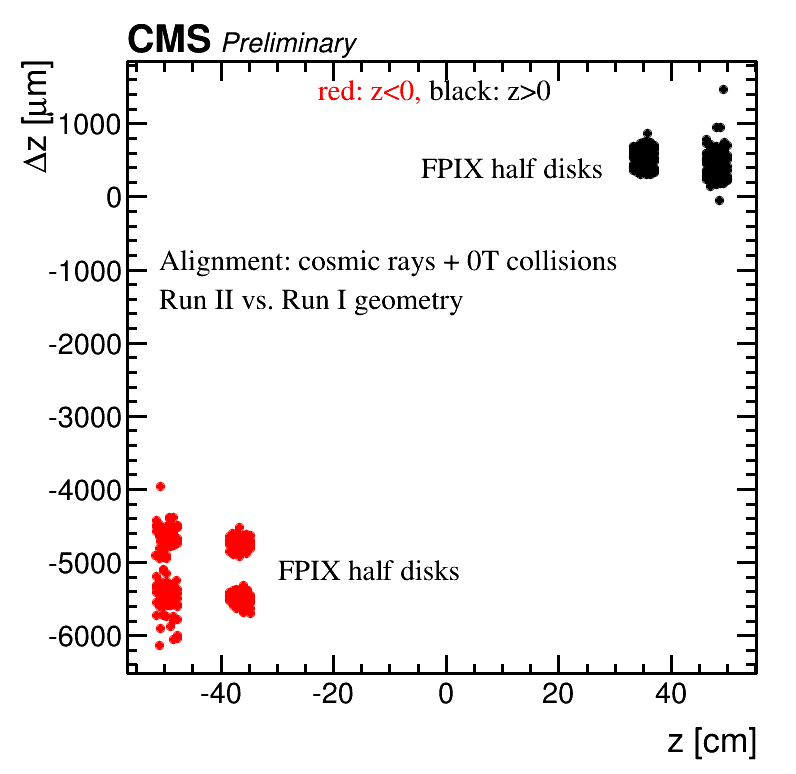
\includegraphics[width=0.45\textwidth]{../figs/Alignment/AlRes_z_vs_dz_PXF_1.png}
    \end{center}
    \caption{Comparison of Run II and Run I positions of the modules in the forward-pixel (FPIX) detector of the tracker, determined with the Millepede-II and HIP algorithms using cosmic ray data collected with $B=0$T and $B=3.8$T magnetic field in the solenoid. The difference $\Delta z$ (Run~II~-~Run~I) as a functions of $z$ (left) and $\phi$ (right) in global coordinates.}
    \label{fig:GCP_FPIX}
\end{figure}

\begin{figure}[htb]
    \begin{center}
        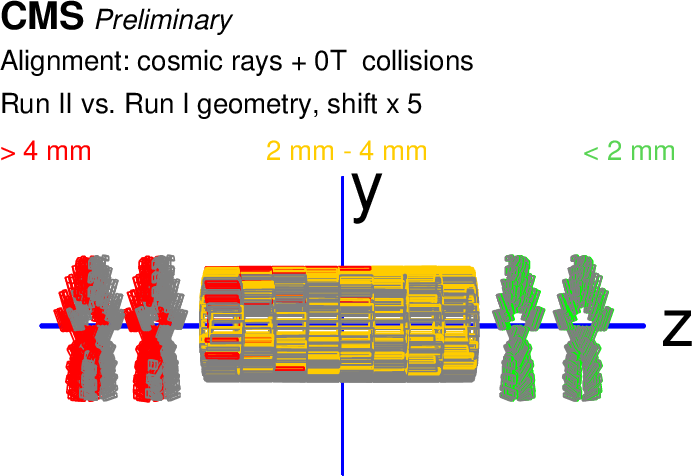
\includegraphics[width=0.95\textwidth]{../figs/Alignment/AlRes_RunIIvsRunI.png}
    \end{center}
    \caption{3D comparison of Run~II and Run~I positions of the pixel modules of the tracker, determined with the Millepede-II and HIP algorithms using cosmic ray data collected with $B=0$T and $B=3.8$T magnetic field in the solenoid and $B=0$T collision data at $\sqrt{s}=13$~TeV. The positions at the end of Run~I are shown in gray. The module shifts between Run~I and Run~II are magnified by a factor of~5 for visualization, and the resulting positions are shown in red, yellow, or green, depending on the magnitude of the shift. }
    \label{fig:GCP_3D}
\end{figure}

\subsection{Distributions of Medians of Unbiased Track-Hit Residuals}
\label{sec:AlRes_DMRs}

Besides geometry comparison, we also have distributions of medians of unbiased track-hit residuals (DMR) validation tool. Each track is refitted using the alignment constants under consideration, and the hit prediction for each module is obtained from all of the other track hits. The median of the distribution of unbiased hit residuals is then taken for each module and is histogrammed. The width of this DMR is a measure of the statistical precision of alignment results; deviations from zero indicate possible biases. The width also has an intrinsic component due to the limited number of tracks, meaning that distributions can only be compared if they are produced with the same number of tracks, as is the case within each set of plots here. 

The DMRs in the transverse plane and in the longitudinal direction are studied in bins of track azimuth $\phi$ and pseudo-rapidity $\eta$. Random misalignments of the modules affect only the resolution of the unbiased track-vertex residual, increasing the width of the distributions, but without biasing their mean. Systematic movements of the modules will bias the distributions in a way that depends on the nature and size of the misalignment and the and of the selected tracks.

The DMRs are plotted for the local x-direction (Fig.~\ref{fig:DMRs}, left) and for the local $y$-direction (Fig.~\ref{fig:DMRs}, right) in the barrel pixel detector, using~2 million cosmic ray tracks collected with the magnetic field at $B=3.8$T. The blue line shows the Run~I geometry, which is no longer valid for Run~II data, primarily because of temperature changes and pixel re-centering and repair. The alignment shown in green was produced with the Millepede-II and HIP algorithms using $B=0$T and $B=3.8$T cosmic ray data. The RMS values, calculated using modules both inside and outside the plot range, show improvement over the Run~I geometry by a factor of~10.

\begin{figure}[htb]
    \begin{center}
        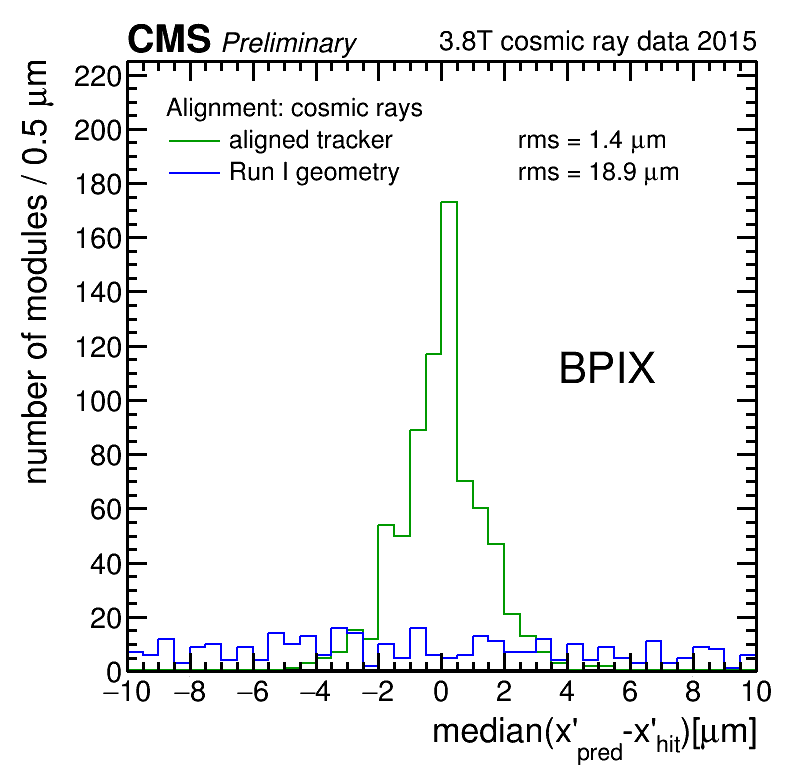
\includegraphics[width=0.45\textwidth]{../figs/Alignment/AlRes_CRAFT_DmedianR_BPIX_plain.png}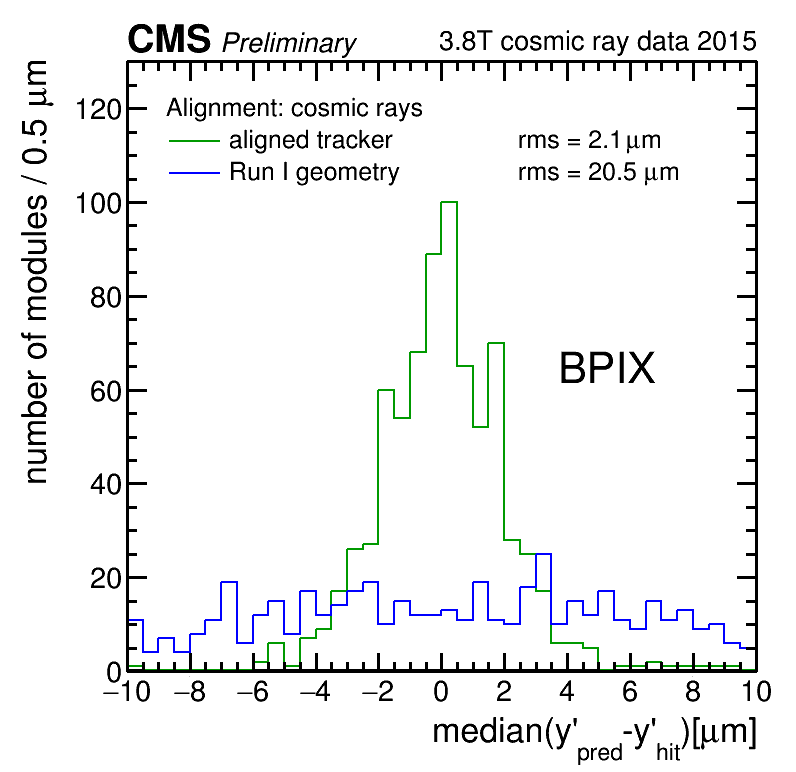
\includegraphics[width=0.45\textwidth]{../figs/Alignment/AlRes_CRAFT_DmedianYR_BPIX_plain.png}
    \end{center}
    \caption {DMRs for the local $x$-direction (left) and for the local $y$-direction (right) in the barrel pixel detector, using~2 million cosmic ray tracks collected with the magnetic field at $B=3.8$T. The blue line shows the Run~I geometry. The alignment shown in green was produced with the Millepede-II and HIP algorithms using $B=0$T and $B=3.8$T cosmic ray data.}
    \label{fig:DMRs}
\end{figure}

\subsection{Cosmic Track Splitting Validation}
\label{sec:AlRes_trackSplit}

Cosmic ray tracks are split in half at the hit closest to origin and refitted with the alignment constants under consideration. The differences in various track parameters between the two half-tracks are studied. The width of the distribution measures the achieved alignment precision, while deviations from zero indicate possible biases. 

Results of the cosmic track splitting validation are shown in Fig.~\ref{fig:trackSplit}. The normalized differences between two halves of a cosmic track, split at the point of closest approach to the interaction region, in $d_{xy}$ (Fig.~\ref{fig:trackSplit}, left), the $xy$ distance between the track and the origin, and in $d_z$ (right), the distance in the $z$ direction between the track and the origin. The observed precision using the aligned geometry (green circles), produced with the Millepede-II and HIP algorithms using cosmic ray data at $B=0$T and $B=3.8$T, is a major improvement over the Run~I geometry (blue empty squares). The precision comes close to that of the ideal Monte Carlo, illustrating that the tracker has almost reached its design spatial resolution.

\begin{figure}[htb]
    \begin{center}
        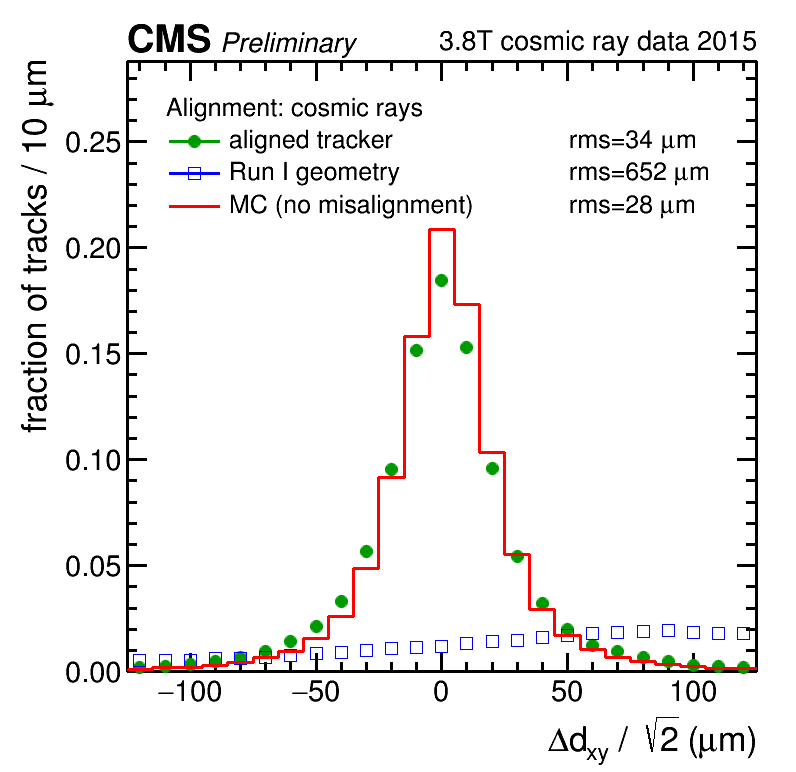
\includegraphics[width=0.45\textwidth]{../figs/Alignment/AlRes_CRAFT_hist_Delta_dxy.png}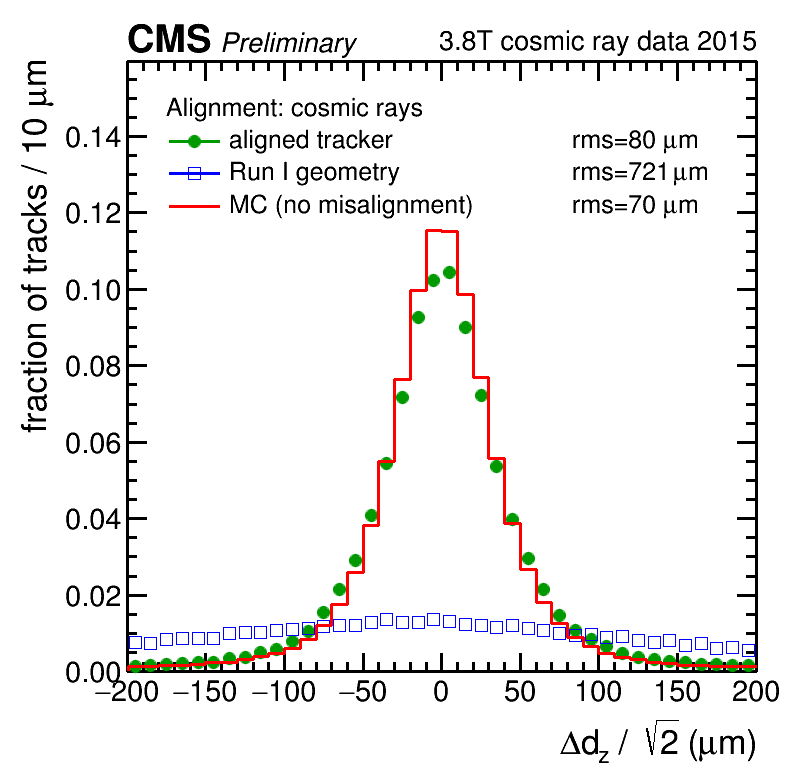
\includegraphics[width=0.45\textwidth]{../figs/Alignment/AlRes_CRAFT_hist_Delta_dz.png}
    \end{center}
    \caption{Cosmic track splitting validation. The normalized differences between two halves of a cosmic track, split at the point of closest approach to the interaction region, in $d_{xy}$ (left), the $xy$ distance between the track and the origin, and in $d_z$ (right), the distance in the $z$ direction between the track and the origin. Aligned geometry (green circles) is produced with the Millepede-II and HIP algorithms using cosmic ray data at~$B=0$T and~$B=3.8$T.}
    \label{fig:trackSplit}
\end{figure}

\subsection{Primary Vertex Validation}
\label{sec:AlRes_PVvalid}

The resolution of the reconstructed vertex position is driven by the pixel detector since it is the closest detector to the interaction point and has the best hit resolution. The primary vertex residual method is based on the study the distance between the track and the vertex, the latter reconstructed without the track under scrutiny (unbiased track-vertex residual). 

The distance in the transverse plane of the track at its closest approach to a refit unbiased primary vertex (Fig.~\ref{fig:PVvalidation}) is studied in bins of track azimuth $\phi$ using a sample of around~5.5M events collected by the CMS detector at zero magnetic field ($B=0$T) selected online through minimum bias triggers. The performance of a dedicated alignment achieved with the Millepede-II and HIP algorithms using cosmic ray data collected with~$B=0$T and~$B=3.8$T magnetic field and~$B=0$T collision data is compared to the one of a previous alignment reached during the commissioning phase with cosmic ray tracks at full magnetic field and to a detailed detector simulation with perfect alignment and calibration. The structures of the green curve indicate relative movements of the pixel half-barrels.

\begin{figure}[htb]
    \begin{center}
        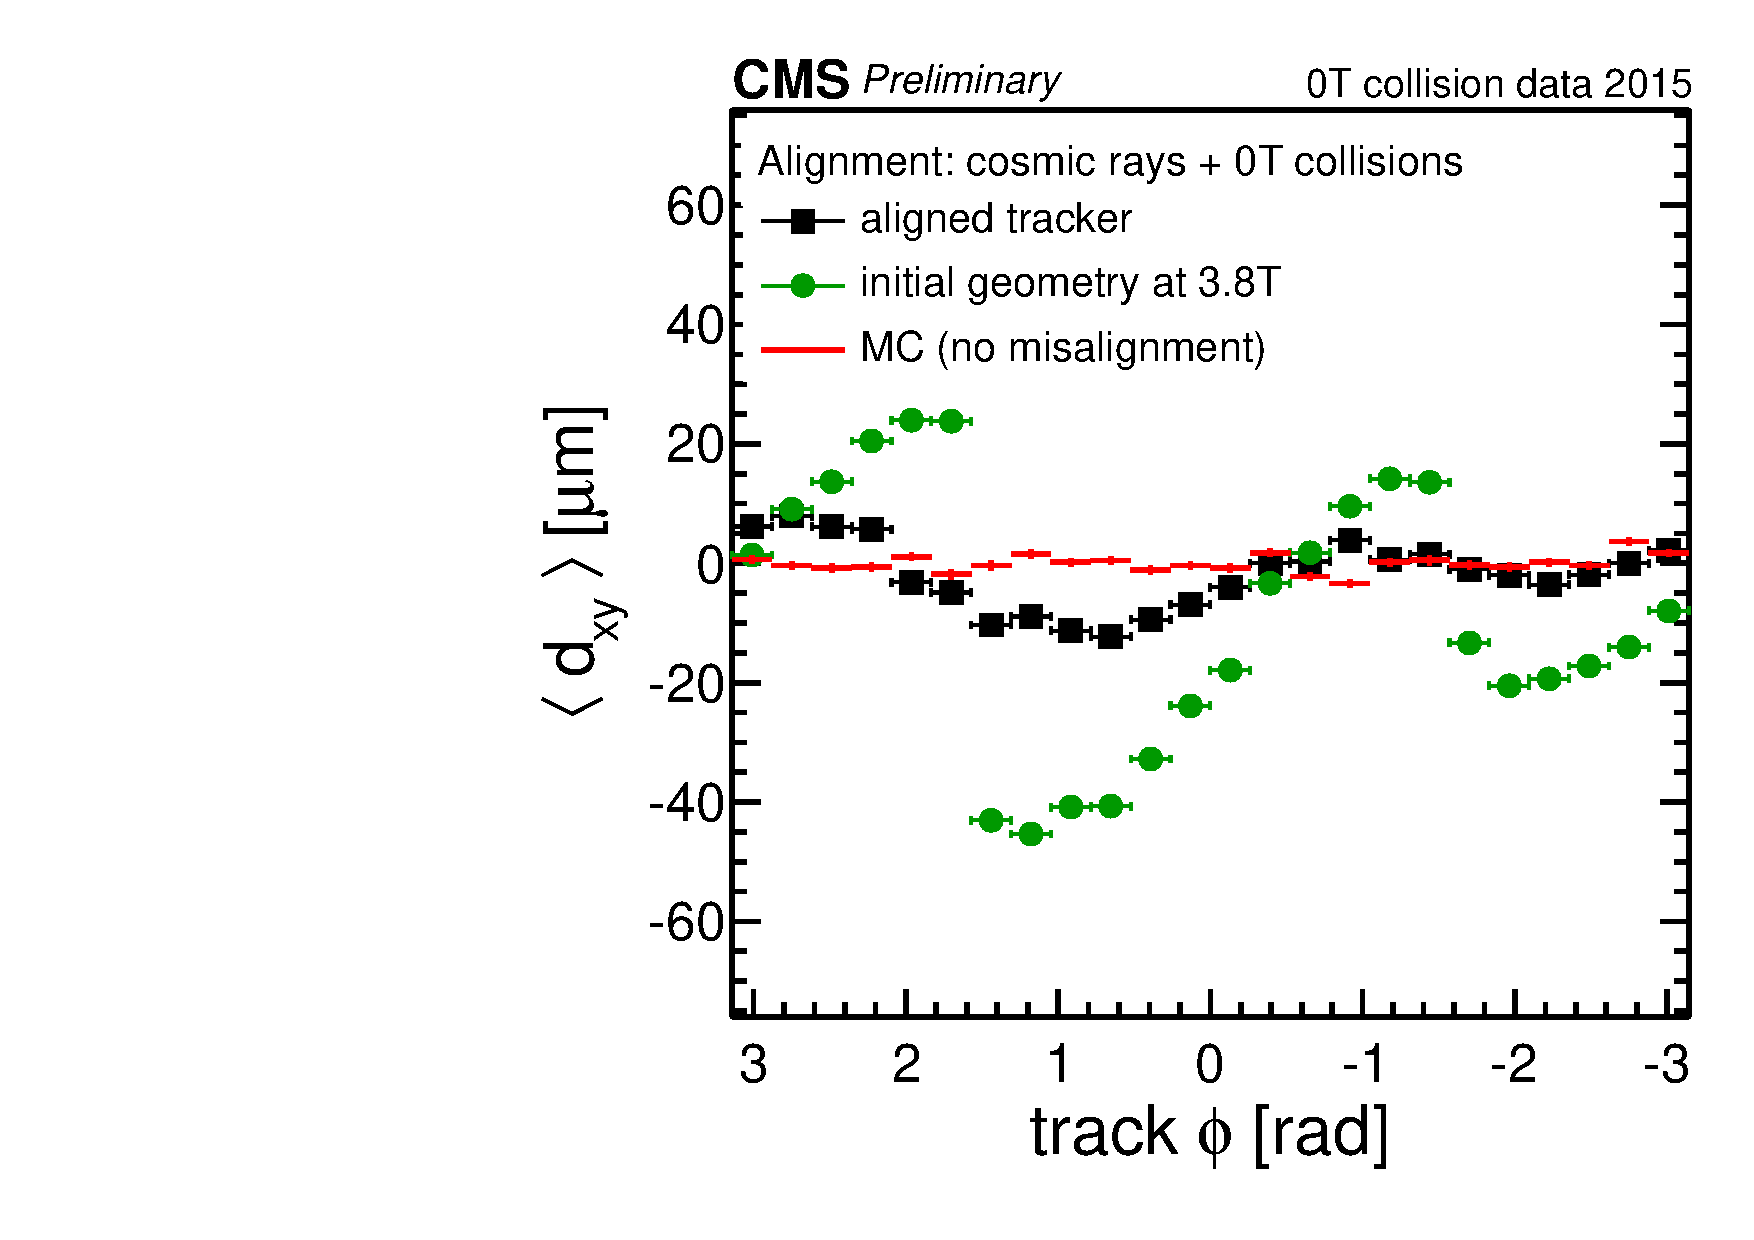
\includegraphics[width=0.45\textwidth]{../figs/Alignment/AlRes_dxyPhiBiasCanvas.pdf}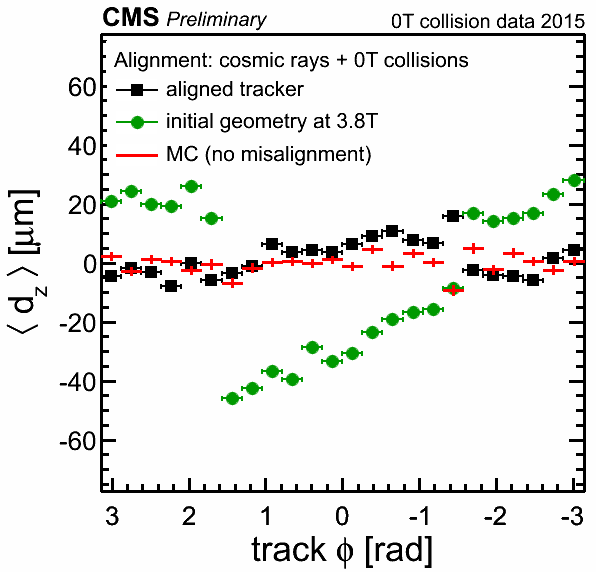
\includegraphics[width=0.45\textwidth]{../figs/Alignment/AlRes_dzPhiBiasCanvas.png}
    \end{center}
    \caption{Primary Vertex Validation. The distance in the transverse plane of the track at its closest approach to a refit unbiased primary vertex ($d_{xy}$, left and $d_z$, right) in bins of track azimuth $\phi$. Validated with CMS data at $B=0$T. Aligned with the Millepede-II and HIP algorithms using cosmic ray data collected with~$B=0$T and~$B=3.8$T magnetic field and $B=0$T collision data. }
    \label{fig:PVvalidation}
\end{figure}

%\begin{figure}[htb]
%    \begin{center}
%        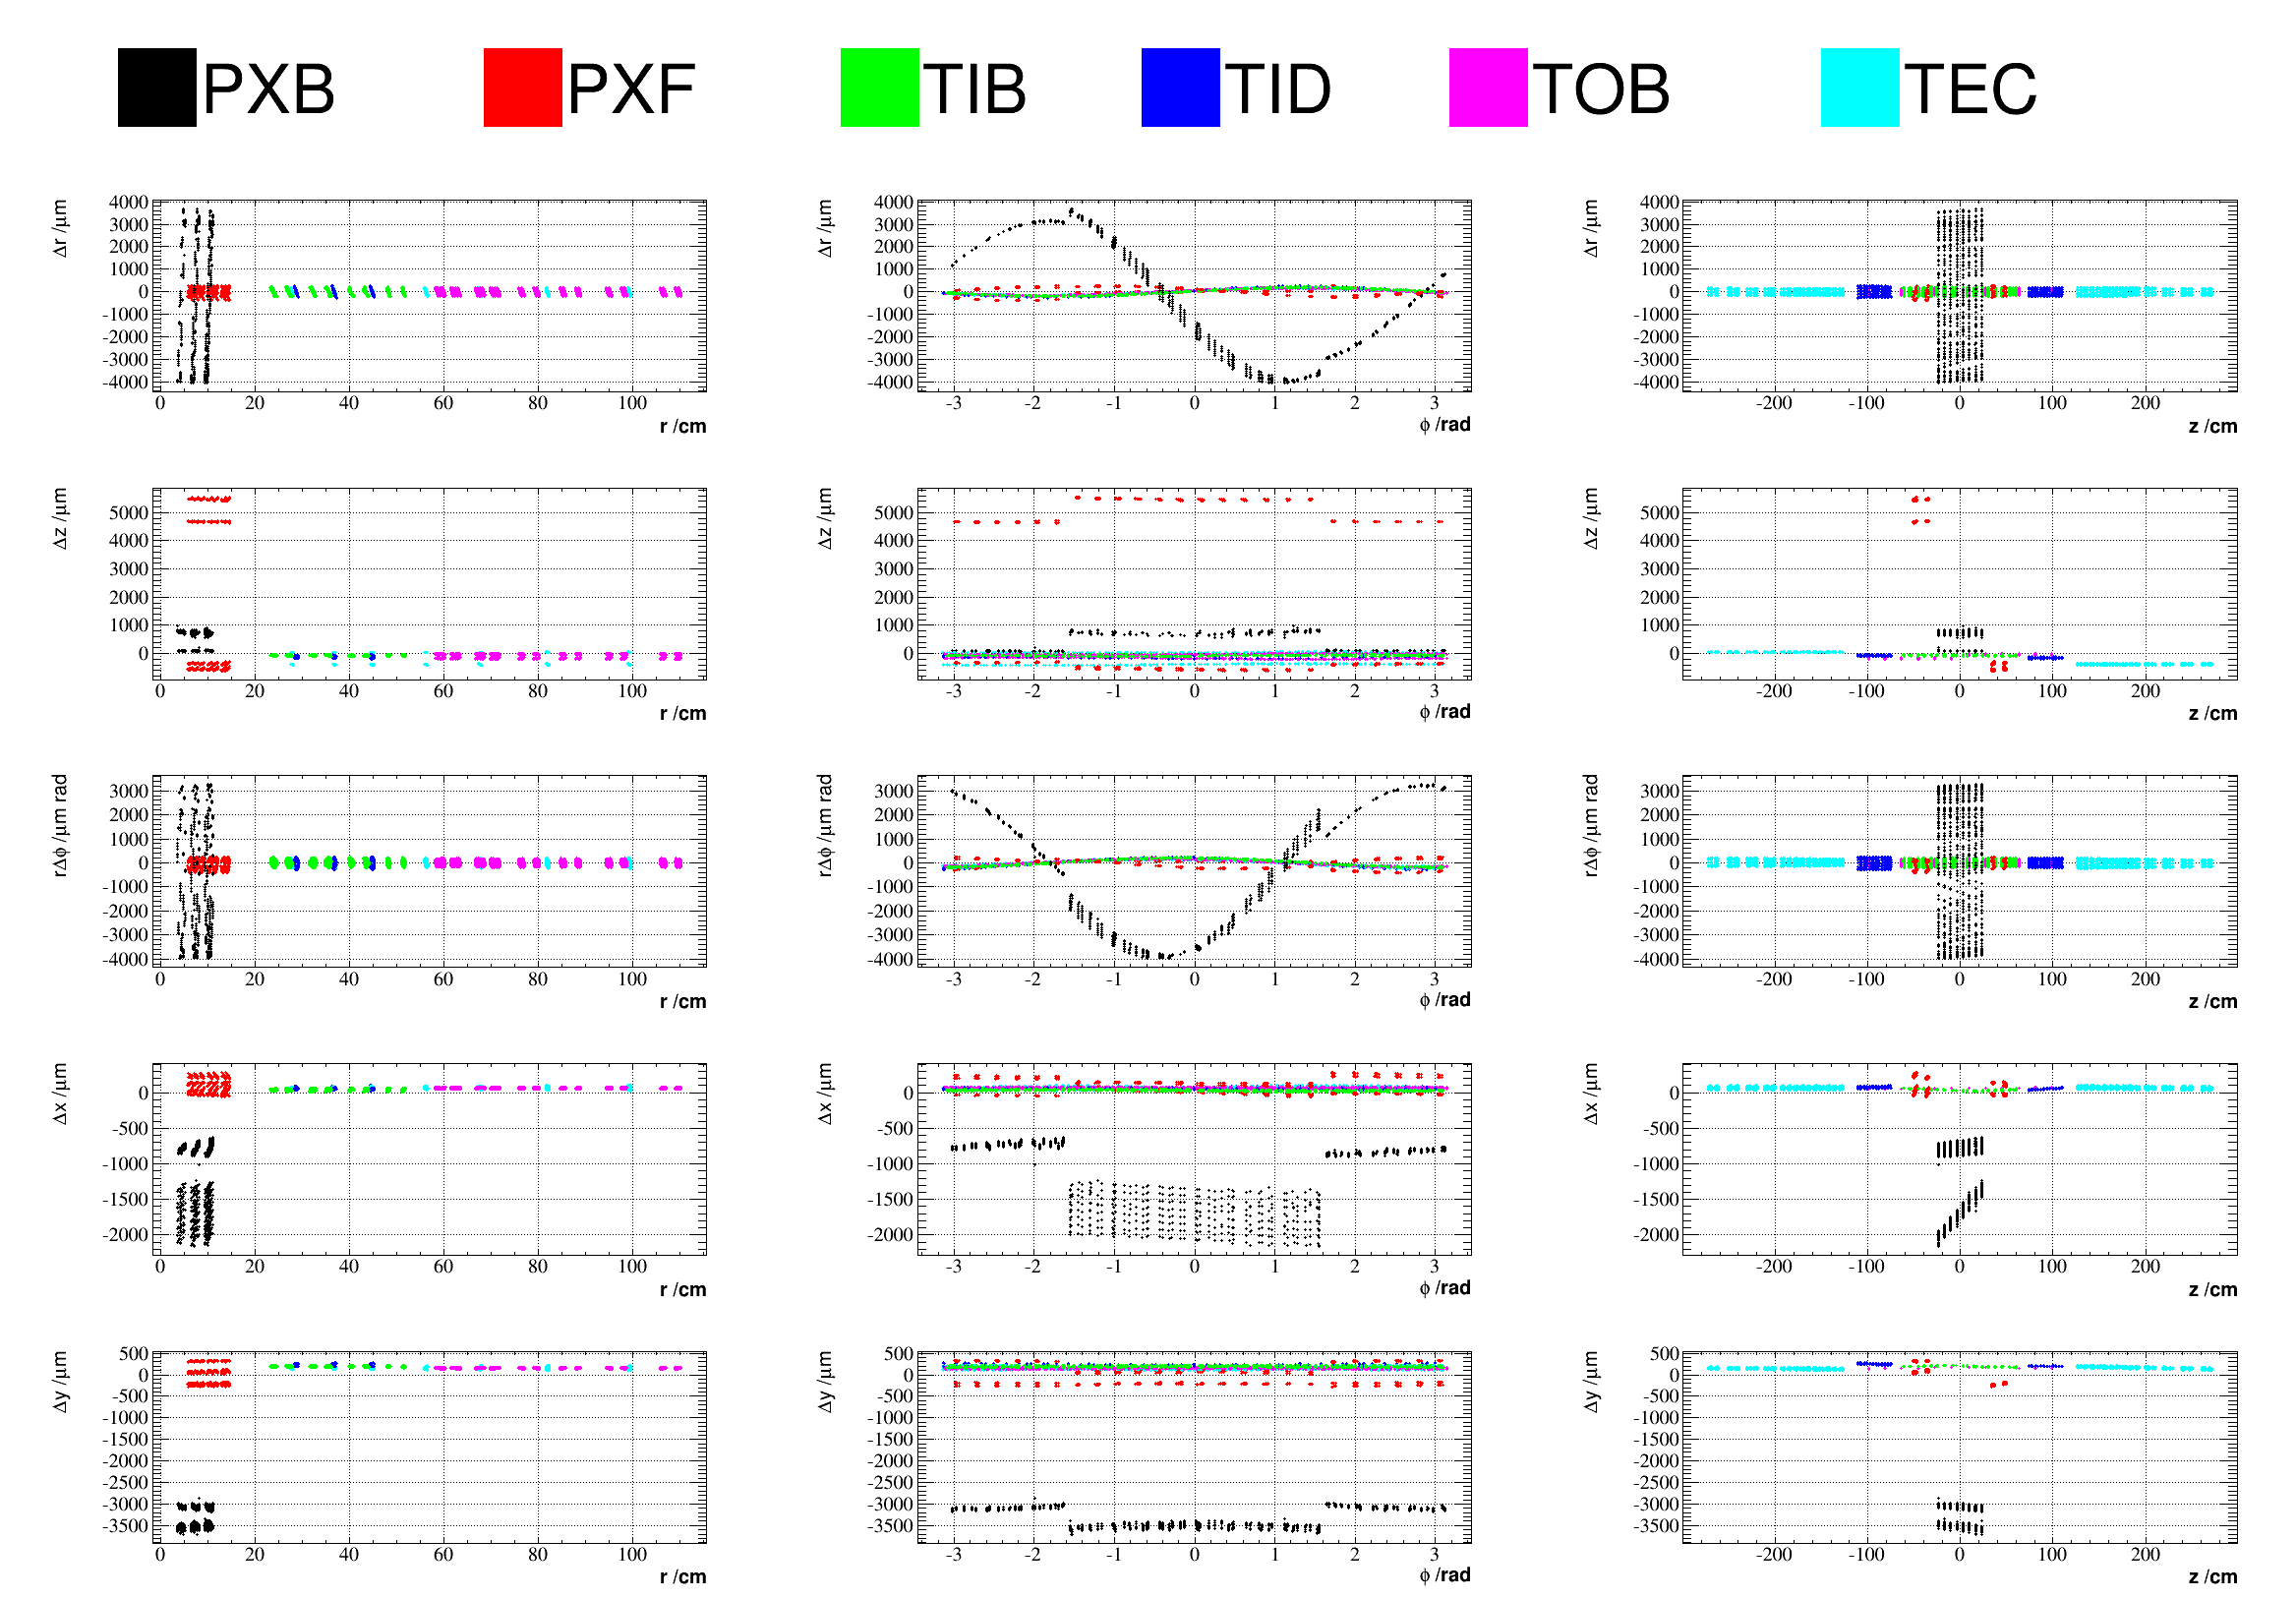
\includegraphics[width=0.98\textwidth]{../figs/Alignment/global_tracker_2_final.png}
%    \end{center}
%    \caption{Geometry comparison plot of CRUZET 2015 object vs Run I.}
%    \label{fig:trackAndResiduals}
%\end{figure}

Given the complexity of the CMS detector, any single measurement based on CMS data requires excellent understanding of the geometry and response of all systems to particles of all types. The CMS Alignment and Calibration team coordinates hundreds of CMS physicists who are working on various aspects of this. The Chapter~\ref{sec:alignment} of this dissertation presented one aspect of this work that concerns alignment of one system of CMS, the part in which the author of this dissertation played an important role.
